\documentclass[conference,a4paper]{IEEEtran}
\IEEEoverridecommandlockouts

\usepackage{cite}
\usepackage{amsmath,amssymb}
\usepackage{graphicx}
\usepackage{array}
\usepackage{booktabs}
\usepackage{url}
\usepackage{tikz}
\usetikzlibrary{positioning,fit,arrows.meta,calc}

\begin{document}

\title{Design of the AI Gateway for the Serbian AI Factory Antenna: Functions and Possible Tools%
\thanks{This work has received funding from the European High Performance Computing Joint Undertaking (JU) under Grant Agreement No.~101263280 (SAIFA).}}

\author{
\IEEEauthorblockN{Aleksandra Stojanovi\'c}
\IEEEauthorblockA{\textit{School of Electrical Engineering} \\
\textit{University of Belgrade}\\
Belgrade, Serbia \\
sa230234d@student.etf.bg.ac.rs}
\and
\IEEEauthorblockN{Dimitrije Pe\v{s}i\'c}
\IEEEauthorblockA{\textit{School of Electrical Engineering} \\
\textit{University of Belgrade}\\
Belgrade, Serbia \\
pd230014d@student.etf.bg.ac.rs}
\and
\IEEEauthorblockN{Zaharije Radivojevi\'c}
\IEEEauthorblockA{\textit{School of Electrical Engineering} \\
\textit{University of Belgrade}\\
Belgrade, Serbia \\
zaki@etf.rs}
}

\maketitle
\bstctlcite{IEEEexample:BSTcontrol}

\begin{abstract}
The EuroHPC AI Factories initiative is building a network of AI supercomputing centres in Europe. AI Factory Antennas bring these services to countries that do not have large AI infrastructure of their own. This paper describes the design of the AI Gateway of the Serbian AI Factory Antenna (SAIFA). The Gateway is the single entry point where researchers, companies, public institutions and students can use national computing resources, datasets, models, workflows, training and support. It also connects these resources with the Pharos and IT4LIA AI Factories. The Gateway is planned as a set of connected components, not as one large platform. We list its main functions, describe each of them, and give possible open-source tools for each part. We also explain which parts have to be developed for SAIFA, how tools will be selected, and what the first test setup for the beta version will include.
\end{abstract}

\begin{IEEEkeywords}
AI Factory, AI gateway, EuroHPC, high-performance computing, MLOps, federation, science gateway.
\end{IEEEkeywords}

\section{Introduction}

Modern artificial intelligence (AI) research needs large computing resources. To give such resources to more users in Europe, the EuroHPC Joint Undertaking started the AI Factories initiative. An AI Factory is a site with an AI supercomputer and services for data, models, training and user support~\cite{eurohpc_aif}. In October 2025, 13 AI Factory Antennas were selected to bring these services to more countries. Each Antenna is linked to one or more AI Factories~\cite{eurohpc_antennas}.

The Serbian AI Factory Antenna (SAIFA) is one of them~\cite{cordis_saifa}. The project runs from May 2026 to April 2029. It uses two national systems: the PARADOX HPC cluster at the Institute of Physics Belgrade and the AI computing infrastructure of the Institute for AI Research and Development of Serbia (ITE). SAIFA is linked with the Pharos (Greece) and IT4LIA (Italy) AI Factories. It focuses on four domains: language and culture, energy and manufacturing, health, and environment.

Users access SAIFA through the \emph{AI Gateway}. Science gateways have been used for years to give users simple access to grid and HPC resources~\cite{wilkinsdiehr2007}. The AI Gateway has the same goal, but it also has to support the whole process of building an AI model and has to work together with partner AI Factories. This paper is based on the first Gateway design~\cite{saifa_d31}. We explain where the Gateway fits in the AI Factory network, list its functions, describe the main ones, and give possible tools and a way to choose between them.

\section{AI Factories, Antennas and the Role of the Gateway}

AI Factories are built around EuroHPC supercomputers. They offer computing power, data, environments for model development, training and expert help~\cite{eurohpc_aif}. Antennas do not copy this infrastructure. They offer a national entry point, local experts and smaller computing resources, and they send larger jobs and finished results to the linked AI Factories. European AI resources can also be found on the AI-on-Demand Platform~\cite{aiod}.

SAIFA is organised in four layers (Fig.~\ref{fig:structure}). The \emph{infrastructure} layer has the compute and storage resources of PARADOX and ITE, which will be connected by a 100\,Gb/s link set up with AMRES. The \emph{computing environment} layer offers AI frameworks in containers and notebooks. The \emph{AI Gateway} layer gives access to models, datasets, tools, workflows, applications, training and support. The \emph{use case} layer holds the domain applications made in the project. Development and first tests are done on national resources. Final tests and benchmarks will be done on the Greek and Italian AI Factories.

\begin{figure}[t]
\centering
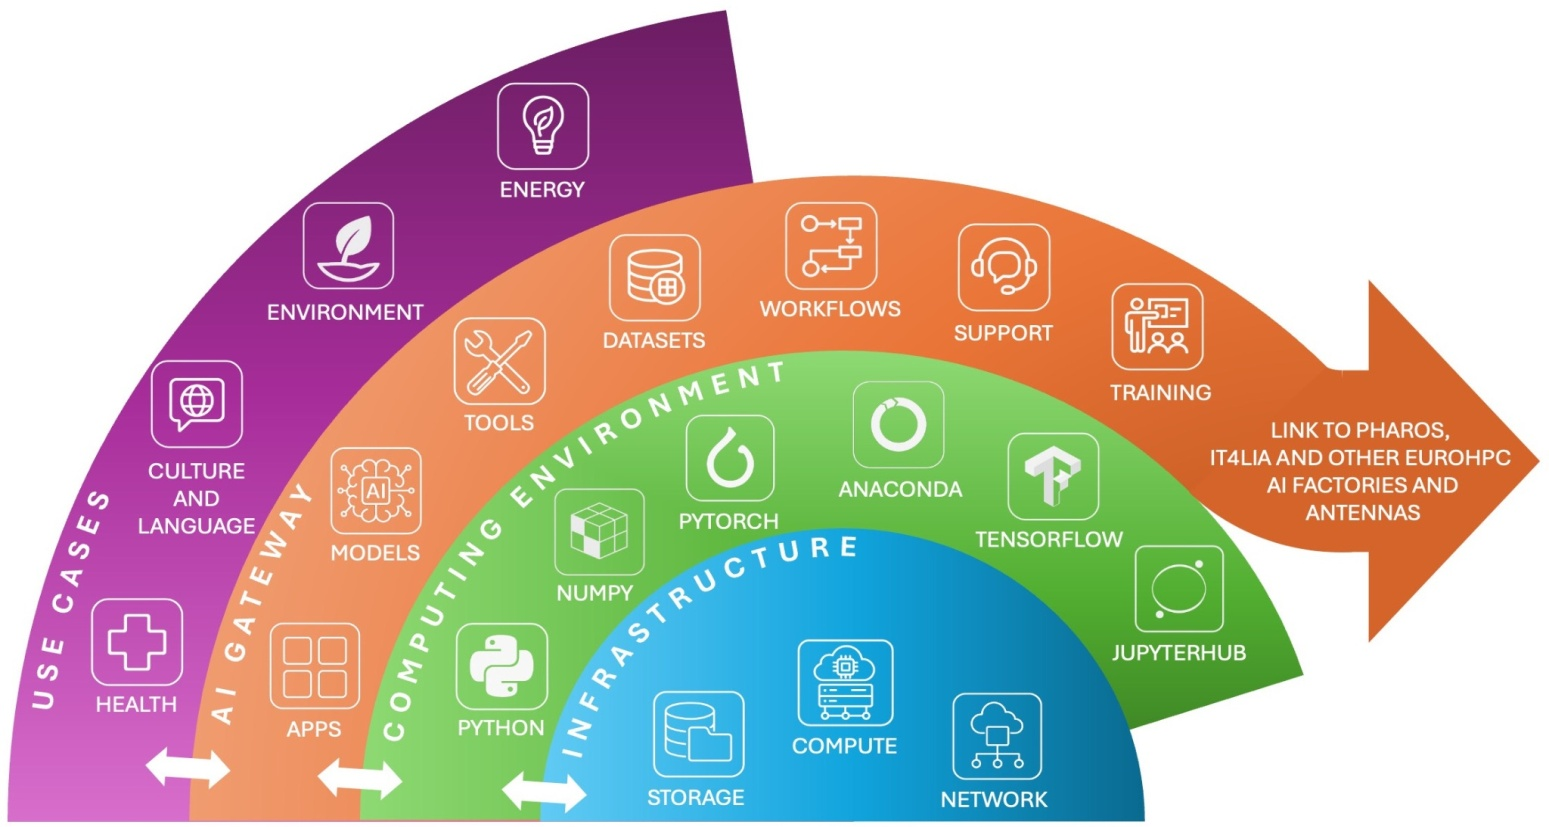
\includegraphics[width=\columnwidth]{fig_saifa_structure.jpg}
\caption{Layered structure of the Serbian AI Factory Antenna.}
\label{fig:structure}
\end{figure}

The Gateway works as \emph{middleware} (Fig.~\ref{fig:arch}). It receives requests from users or applications, applies the same rules for identity, access and metadata to all of them, and sends each request to the right service. The Gateway handles login and access control, the catalogue, checking and routing of requests, quotas, job status, monitoring, audit logs and data origin. It does not replace schedulers, clusters, storage systems, model servers or learning systems. Domain logic, data preparation and the meaning of results stay with the domain applications or with the users' own code.

\begin{figure}[t]
\centering
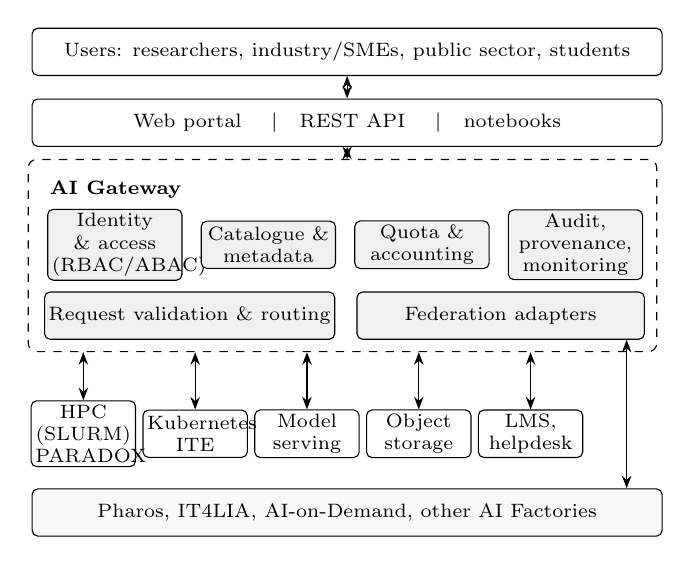
\begin{tikzpicture}[
  font=\scriptsize,
  box/.style={draw, rounded corners=2pt, align=center, minimum height=6mm, inner sep=1.5pt},
  core/.style={box, fill=gray!12},
  >={Stealth[length=1.6mm]}
]
% user-facing rows (total width 8.0 cm)
\node[box, minimum width=8cm] (users) at (4,0) {Users: researchers, industry/SMEs, public sector, students};
\node[box, minimum width=8cm] (portal) at (4,-0.9) {Web portal \quad\textbar\quad REST API \quad\textbar\quad notebooks};
% gateway core
\node[font=\scriptsize\bfseries, anchor=west] (gwt) at (0.1,-1.75) {AI Gateway};
\node[core, text width=1.6cm] (iam)   at (1.05,-2.45) {Identity \& access\\(RBAC/ABAC)};
\node[core, text width=1.6cm] (cat)   at (3.0,-2.45) {Catalogue \&\\metadata};
\node[core, text width=1.6cm] (quota) at (4.95,-2.45) {Quota \&\\accounting};
\node[core, text width=1.6cm] (audit) at (6.9,-2.45) {Audit, provenance,\\monitoring};
\node[core, minimum width=3.65cm] (route) at (2.0,-3.35) {Request validation \& routing};
\node[core, minimum width=3.65cm] (fed)   at (5.95,-3.35) {Federation adapters};
\node[draw, dashed, rounded corners=3pt, fit=(gwt)(iam)(audit)(route)(fed), inner sep=1.5mm] (gw) {};
% back-ends (x from 0 to 7.0 cm)
\foreach \n/\x/\t in {hpc/0.65/{HPC (SLURM)\\PARADOX}, k8s/2.07/{Kubernetes\\ITE}, serve/3.49/{Model\\serving}, store/4.91/{Object\\storage}, lms/6.33/{LMS,\\helpdesk}}
  \node[box, minimum width=1.3cm, text width=1.22cm] (\n) at (\x,-4.85) {\t};
\node[box, minimum width=8cm, fill=gray!5] (aif) at (4,-5.85) {Pharos, IT4LIA, AI-on-Demand, other AI Factories};
% links
\draw[<->] (users) -- (portal);
\draw[<->] (portal) -- (portal |- gw.north);
\foreach \n in {hpc,k8s,serve,store,lms} \draw[<->] (gw.south -| \n) -- (\n);
\draw[<->] (7.55,-3.35 |- fed.south) -- (7.55,-3.35 |- aif.north);
\end{tikzpicture}
\caption{The AI Gateway between users, national resources and partner AI Factories.}
\label{fig:arch}
\end{figure}

\section{Gateway Functions}

We started from the users. First, we wrote 23 user stories for the four domains and for general use. Examples are forecasting of renewable energy, optimisation of industrial processes with surrogate models, flood prediction with AutoML, synthetic genome sequencing data, early disease detection, hate-speech detection in Serbian and simulation of social networks with LLM agents. Each story lists who the users are, what they need, what they expect to get and which Gateway functions they use. From these stories we made 20 system use cases. Each use case has actors, preconditions, a main flow, alternative flows and a final state.

All functions used in the stories fall into ten groups, shown in Table~\ref{tab:func}. Three rules apply to all of them: the server checks permissions for every action, every result has a version and a record of where it came from, and every job is checked against the user's quota before it starts.

\begin{table}[t]
\centering
\caption{Main function groups of the AI Gateway}
\label{tab:func}
\footnotesize
\renewcommand{\arraystretch}{1.1}
\begin{tabular}{@{}p{2.1cm}p{5.9cm}@{}}
\toprule
\textbf{Group} & \textbf{Main features} \\
\midrule
Identity \& access & Institutional (eduGAIN) and EuroHPC sign-in, account linking, RBAC/ABAC, scoped API tokens, revocation \\
Organisations \& projects & Workspaces, membership, roles, resource visibility (private, project, platform, public) \\
Catalogue & Search and filtering of models, datasets, workflows and courses; source attribution of federated resources \\
Data \& model management & Resumable upload, versioning, metadata and model cards, review and publication workflow \\
Compute jobs & Job templates, quota reservation, routing to SLURM or Kubernetes, status, logs, result retrieval \\
Inference & Authenticated, rate-limited access to served models and LLMs \\
Experiments \& MLOps & Experiment tracking, run comparison, benchmark evaluation, lineage across job, dataset and model \\
Training & Courses, learning paths, preconfigured notebook labs with controlled resource templates \\
Operations & Monitoring, usage accounting, audit trail, notifications, contextual helpdesk tickets \\
Federation & Catalogue exchange, metadata mapping, identity brokering, export of approved assets \\
\bottomrule
\end{tabular}
\end{table}

\begin{table*}[t]
\centering
\caption{Possible tools for each part and work needed for SAIFA}
\label{tab:tools}
\footnotesize
\renewcommand{\arraystretch}{1.08}
\begin{tabular}{@{}p{3.0cm}p{7.2cm}p{6.6cm}@{}}
\toprule
\textbf{Part} & \textbf{Main option (alternatives)} & \textbf{Work needed for SAIFA} \\
\midrule
Portal \& UX & Next.js/React (Nuxt/Vue) & SAIFA UI, backend-for-frontend, tool embedding \\
Identity \& SSO & Keycloak (authentik, WSO2 IS) & role mapping, ABAC attributes, account linking \\
Access policies & Open Policy Agent (Casbin, Cedar) & SAIFA RBAC/ABAC policy model \\
Notebooks & JupyterHub + KubeSpawner (SlurmSpawner, code-server) & launch from portal, quotas, dataset mount, audit \\
Catalogue \& search & CKAN or Dataverse (DataHub, OpenMetadata); OpenSearch + pgvector & unified catalogue, ACL filtering in index, federation \\
Model registry \& experiments & MLflow (ClearML, Aim) & model cards, approval workflow, access rights \\
LLM inference \& serving & vLLM (TGI, SGLang, Triton); KServe (Ray Serve, BentoML) & API proxy, quotas, routing, audit \\
Fine-tuning & Hugging Face TRL/PEFT (Axolotl, LLaMA-Factory) & approved templates, HPC submission, result registration \\
HPC \& batch & SLURM on existing clusters, Open OnDemand; Kubernetes Jobs (Volcano, Kueue) & HPC bridge, unified job model, SLURM/K8s routing \\
Workflows & Argo Workflows (Airflow, Flyte, Kubeflow) & simple SAIFA workflow templates \\
Containers & Harbor + Trivy, Apptainer on HPC & image approval and HPC conversion \\
Storage & PostgreSQL, S3-compatible object store (MinIO/Ceph), Valkey & metadata links, lifecycle, retention \\
Observability \& audit & Prometheus, Grafana, Loki, OpenTelemetry; append-only log + WORM archive & correlation with user/job, shared audit events \\
Learning \& support & Moodle (Open edX); Zammad or GLPI & portal links, lab quotas, contextual tickets \\
Lineage & OpenLineage + Marquez & links between jobs, datasets, models and results \\
Federation \& accounting & DCAT/DCAT-AP adapters (CKAN harvester); Waldur as cross-layer option & Pharos/IT4LIA adapters, per-factory accounting \\
\bottomrule
\end{tabular}
\end{table*}

\section{Description of the Main Functions}

\subsection{Login, access and collaboration}
Users log in with their university or institute account through AMRES/eduGAIN, or with a EuroHPC account. The Gateway connects these logins to one user account. Access is decided by the user's role and by other attributes, such as organisation, project and type of data~\cite{nist_abac}. Seeing a resource in the catalogue and using it are two separate permissions. The search index also filters results, so users never see resources they are not allowed to use. A leak of data between projects is treated as a problem that stops a release.

\subsection{Datasets and models}
Datasets and models go through three steps: draft, review and publication. The owner uploads a resource with its licence, domain and language and sends it for review. A data or model reviewer accepts it, rejects it or sends it back for changes, and every decision is saved. Large files are uploaded in parts with checksums, so an upload can continue after a break. Only checked versions that can no longer change can be published or used. Published resources have FAIR metadata~\cite{wilkinson2016fair} and can be sent to external repositories with a permanent identifier.

\subsection{Compute jobs and the HPC bridge}
Users start training, fine-tuning or batch jobs from the portal, the API or a notebook. Before a job starts, the Gateway checks the parameters and the user's access to the input data, and reserves quota. Then it picks where the job will run: SLURM~\cite{yoo2003slurm} on PARADOX for HPC jobs, or Kubernetes~\cite{burns2016borg} for container and interactive services. Sensitive data can stay where it is, and the job is sent to the data. The scheduler still manages the queue. The Gateway collects job status, logs and results and shows them to the user in the same way for all systems. Code that is specific to one cluster is kept in separate adapters, and containers are converted to Apptainer/Singularity images~\cite{kurtzer2017singularity} for HPC.

\subsection{Inference, experiments and evaluation}
Requests to a model go through a Gateway proxy. The proxy checks who is calling, checks access and limits, charges the quota and only then forwards the request to the model server. Training runs save their parameters, metrics and files and link them to the input data and the job. Model versions are tested on benchmarks that also have versions. Users can compare runs, but a person always decides which model to keep. A model can be sent for review only when its test results are attached.

\subsection{Training, support and federation}
Students open ready-made notebook labs with read-only data and run prepared jobs, without working with the scheduler. Help requests are sent from the page where the problem happened, and the job or resource ID is added automatically. Each partner AI Factory is connected through its own catalogue adapter, which converts metadata, for example to DCAT~\cite{w3c_dcat3}. Resources from partners keep their source and are never changed locally. Approved public SAIFA resources can be sent to partner catalogues. The first connections to partners are read-only or simulated, so the Gateway keeps working when a partner is down.

\section{Possible Tools and How to Choose Them}

The main rule is to use existing tools first and build new ones only when needed. Table~\ref{tab:tools} gives the main option for each part, alternatives in brackets, and the work that is specific to SAIFA. Most options are well known open-source projects, for example JupyterHub~\cite{kluyver2016jupyter}, MLflow~\cite{zaharia2018mlflow}, vLLM~\cite{kwon2023vllm} and Open OnDemand~\cite{hudak2018ood}. New development is needed mainly for the portal, the common metadata model, the shared rules for access and quotas, audit and accounting, the HPC bridge and the adapters for partner AI Factories.

Waldur is also considered, because one tool could cover the service catalogue, project resources, accounting and HPC access. It will be compared with a set of separate tools. Using Waldur for one part does not mean it has to be used for the others.

Tools are chosen in two steps. First, each tool must meet the basic requirements for its area. For example, it must support login with SAML2 and OIDC to one account and allow access to be removed at once. The search must filter results by access rights. The model server must run behind the Gateway, and quota must be charged before a request runs. Users must not need to work with SLURM directly, and a new partner must be added with a new adapter. Second, the tools that pass are compared by ease of use, work needed to connect them, effort to run them, speed and cost, maturity, and legal issues (GDPR, data location, licences). Open-source tools that can run on our own servers are preferred. Paid tools and tools with restrictive licences are noted, together with a plan to replace them if needed.

The first test setup for the beta version will include a web portal, login through home institutions, an access-control module, PostgreSQL with S3 storage, JupyterHub, a model-serving service, a separate bridge to SLURM, and Prometheus/Grafana monitoring. For each part, the tests must show where the data is stored, how the user identity is passed on, how resources are charged, how actions are logged, how access is checked and what happens when another service fails.

\section{Plan and Conclusion}

The design was finished in month 3 of the project (July 2026). The beta version of the Gateway and the access rules have to be online in month 12 (April 2027). The beta must offer at least one full path for a user: log in, find a resource, run a job and follow its progress. A report on the finished functions is due in month 18 (October 2027). Work on integration, security and connections with partners continues until April 2029. Each beta function is linked to its risks and tests. A function is not released if a high security, privacy or domain risk remains, even if it works correctly.

This paper presented the AI Gateway of SAIFA. The Gateway connects users in Serbia with national resources and with the EuroHPC AI Factories. It sits between users and existing systems and has clearly defined tasks, so most of its parts can be built from existing open-source tools. New development is focused on the catalogue with access control, quotas and audit, the HPC bridge and the connections to partners. Next, we will check the functions with domain experts, finish the test setups and report on the beta version and on tests with Pharos and IT4LIA.

\bibliographystyle{IEEEtran}
\bibliography{references}

\end{document}
